\documentclass[11pt,compress]{beamer}
% deactivate beamer navigation
%\setbeamertemplate{navigation symbols}{}
%\usepackage{geometry}
%\geometry{papersize={180mm, 135mm}, top=-1.5mm} % 210mm, 297mm
%\PassOptionsToPackage{wide}{../../style/lmu-lecture}
\usepackage{../../style/lmu-lecture}
\setbeamertemplate{frametitle}{\expandafter\uppercase\expandafter\insertframetitle}

\usepackage{tikz}
\usepackage{setspace}

\AtBeginSection[]
{
  \begin{frame}<beamer>
    \frametitle{Introduction to Machine Learning}
    \scriptsize
    \tableofcontents[currentsection, subsectionstyle=hide]
  \end{frame}
}
% includepdf slides, pagecommad will set counter for framenumber
\usepackage{pdfpages}
\includepdfset{
  trim=0mm 0mm 0mm 0mm, 
  pagecommand={\global\setcounter{framenumber}{\value{page}}}
}
% trim=0mm 6mm 0mm 0mm, offset=0 15,
% add footer:
\usepackage{framed, color}
\usepackage{xcolor}
%\iffalse
\setbeamertemplate{footline}[text line]{%
  \noindent\hspace*{\dimexpr-\oddsidemargin-1in\relax}%
  \colorbox{white}{
    \makebox[\dimexpr\paperwidth-2\fboxsep\relax]{
      \color{black}
      \begin{minipage}[c][4.5ex][c]{\linewidth}
      \secname \hfill \insertframenumber{}~/~\inserttotalframenumber~~
        \end{minipage}
    }}%
}
%\fi


\title{
%\centerline{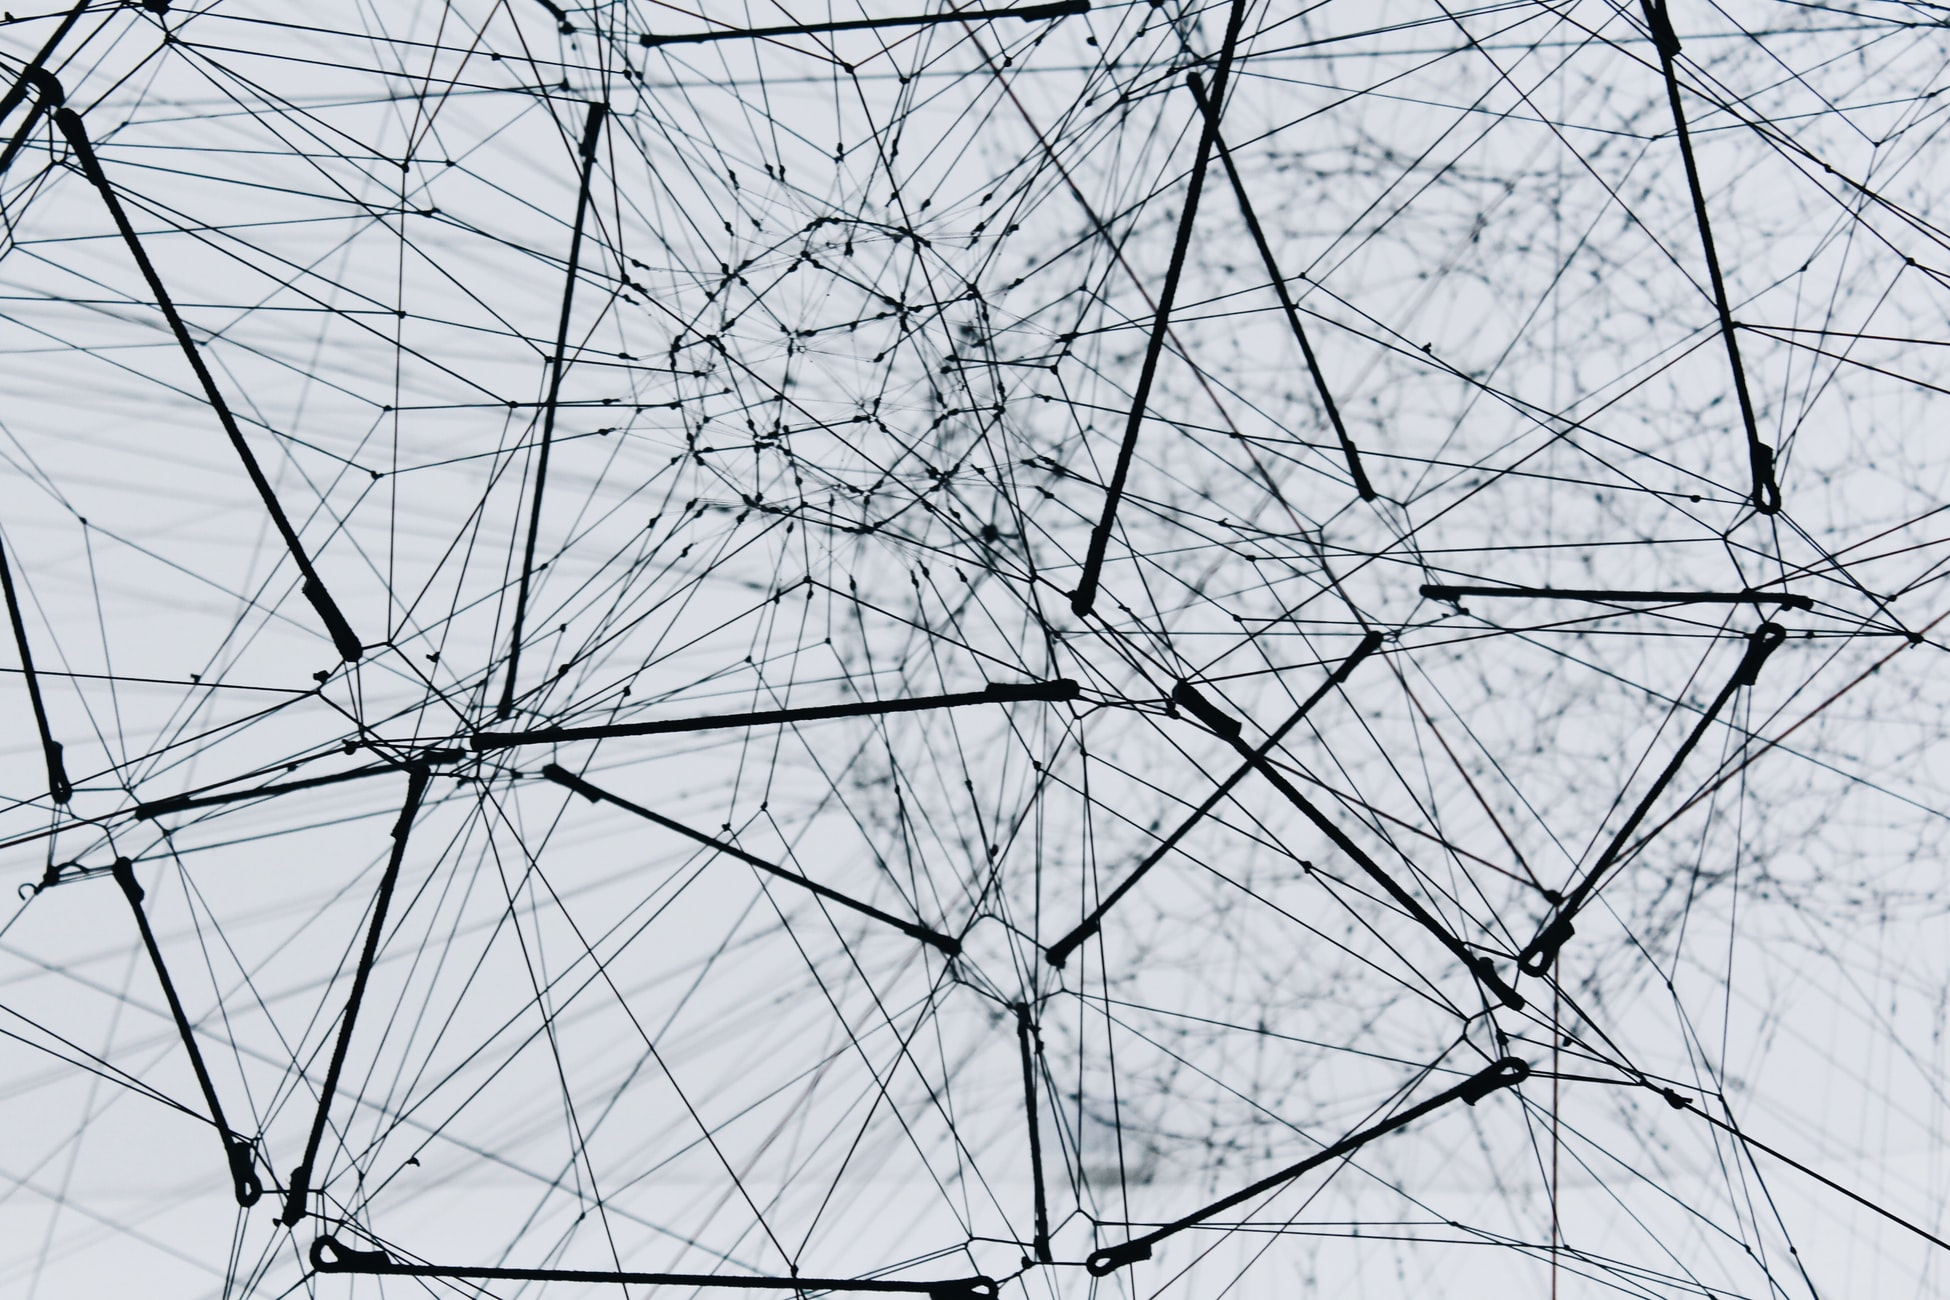
\includegraphics[width=0.75\paperwidth,keepaspectratio, trim={0 15cm 0 5cm}, clip]{titlepage.jpg}}
\centerline{
\includegraphics[width=0.25\paperwidth,]{../../style/logo.pdf}}
\medskip
Introduction to Machine Learning \\
\medskip
\small All slides \\
\bigskip
\small \today
}



\begin{document}
\setbeamercolor{background canvas}{bg=}

\begin{frame}[noframenumbering,plain]
\maketitle
\end{frame}


% General remark: hyperlinks in included pdfs are not clickable anymore in the combined pdf

% Include tuning lecture slides
\section{ML Basics}
%Suggested order of slides
% slides-bayes-lm.tex
% slides-gp-basic.tex
% slides-gp-covariance.tex
% slides-gp-prediction.tex
% slides-gp-training.tex
% slides-gp-mean.tex

% not included: 
% slides-x-covariance-adv.tex
% slides-x-gp-additional.tex
% slides-x-gp-classification.tex

\subsection{Bayes LM}
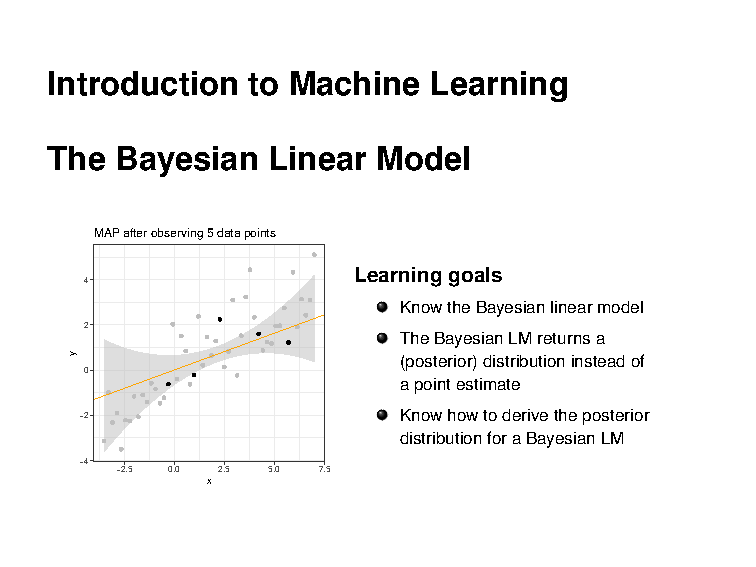
\includepdf[pages=-]{../slides-pdf/slides-gp-bayes-lm.pdf}
\subsection{Gaussian Processes - Basics}
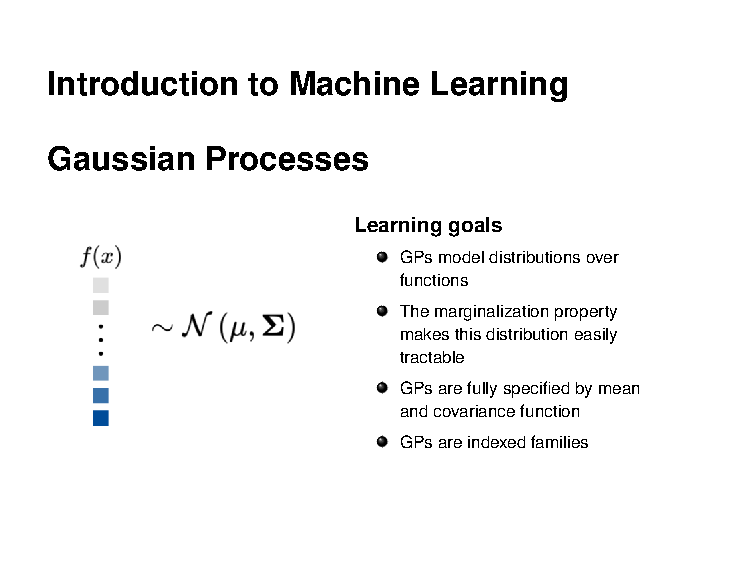
\includepdf[pages=-]{../slides-pdf/slides-gp-basic.pdf}
\subsection{Gaussian Processes - Covariance}
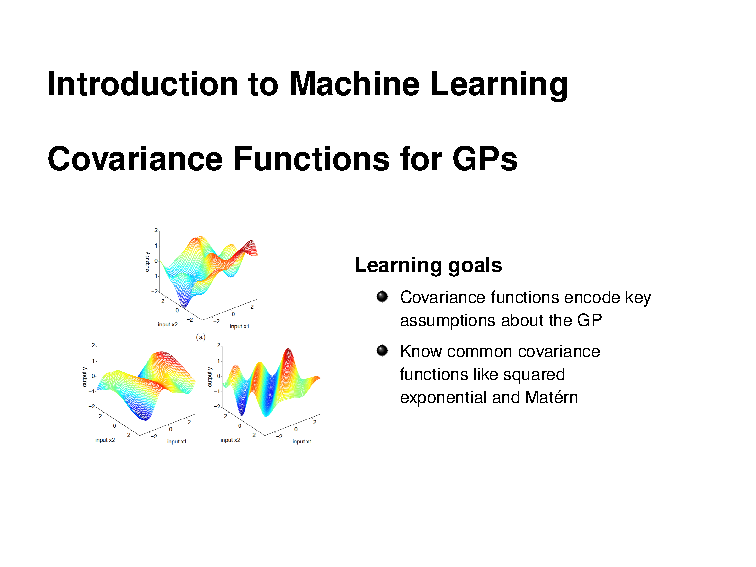
\includepdf[pages=-]{../slides-pdf/slides-gp-covariance.pdf}
\subsection{Gaussian Processes - Prediction}
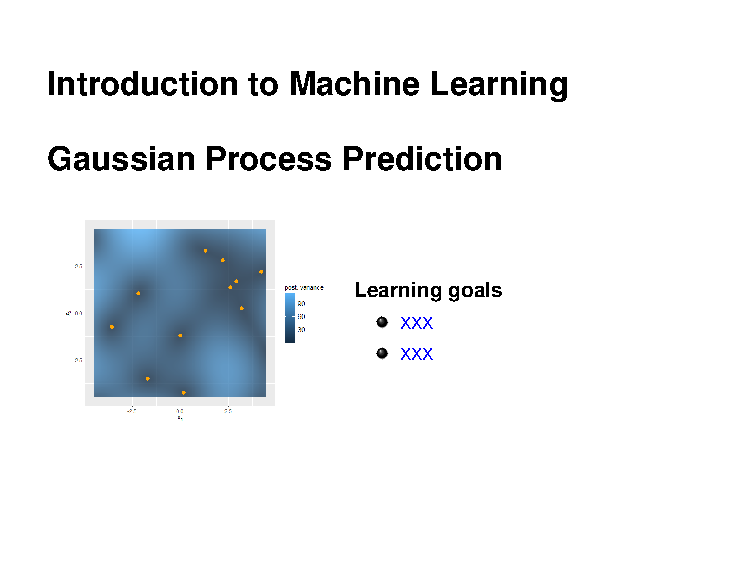
\includepdf[pages=-]{../slides-pdf/slides-gp-prediction.pdf}
\subsection{Gaussian Processes - Training}
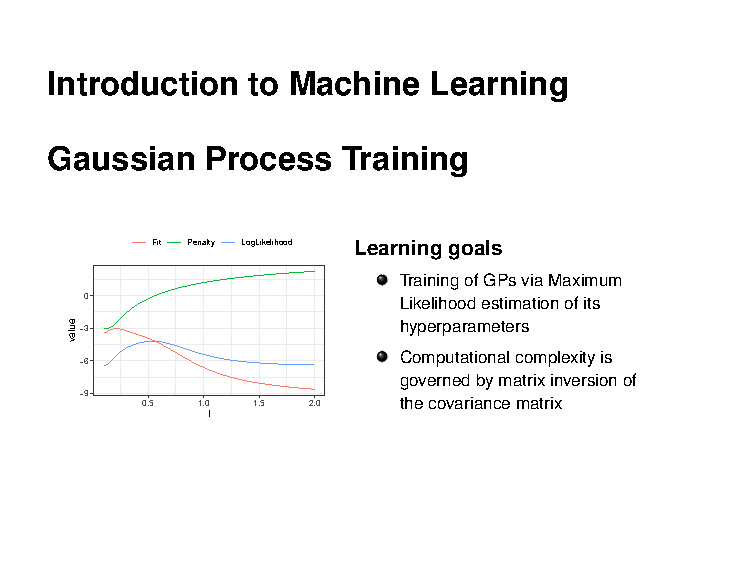
\includepdf[pages=-]{../slides-pdf/slides-gp-training.pdf}
\subsection{Gaussian Processes - Mean}
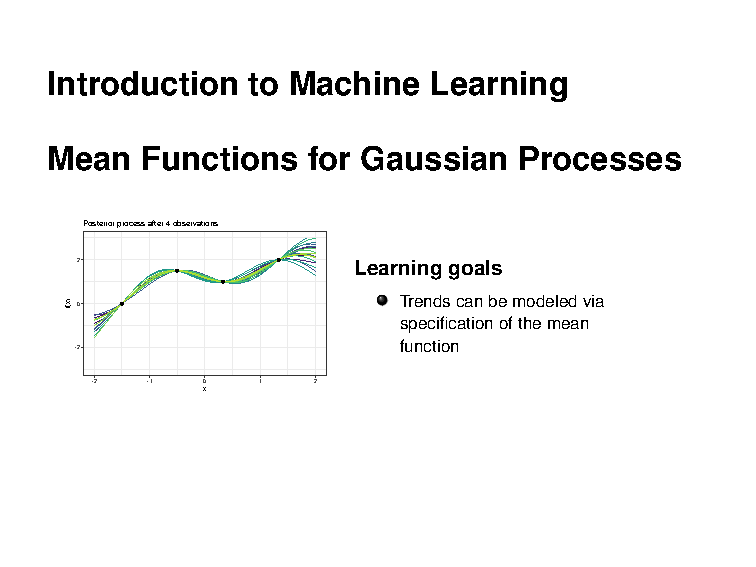
\includepdf[pages=-]{../slides-pdf/slides-gp-mean.pdf}


\section{Supervised Regression}
%Suggested order of slides
% slides-bayes-lm.tex
% slides-gp-basic.tex
% slides-gp-covariance.tex
% slides-gp-prediction.tex
% slides-gp-training.tex
% slides-gp-mean.tex

% not included: 
% slides-x-covariance-adv.tex
% slides-x-gp-additional.tex
% slides-x-gp-classification.tex

\subsection{Bayes LM}
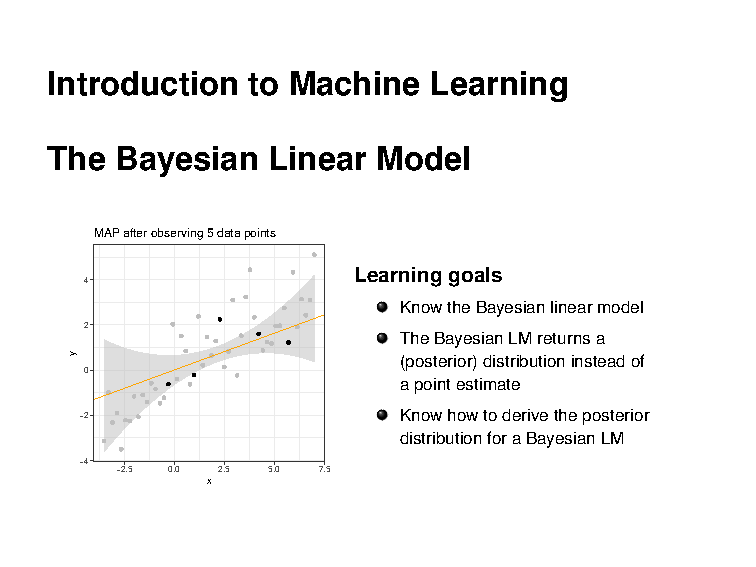
\includepdf[pages=-]{../slides-pdf/slides-gp-bayes-lm.pdf}
\subsection{Gaussian Processes - Basics}
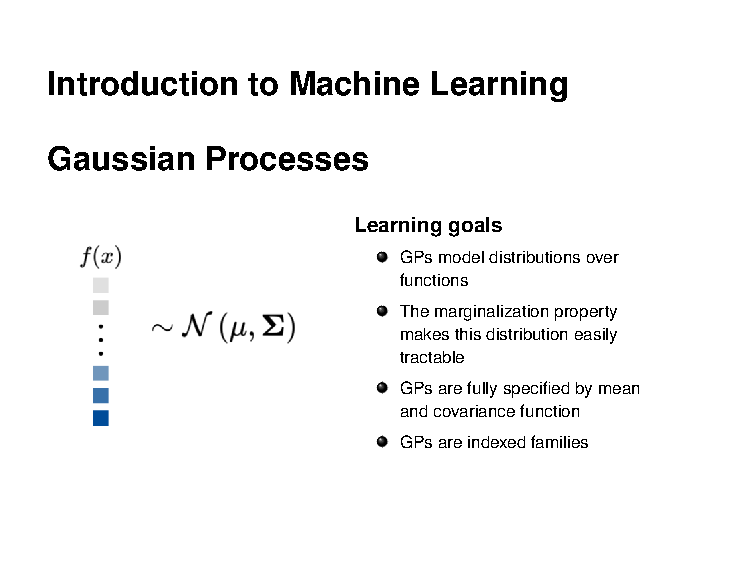
\includepdf[pages=-]{../slides-pdf/slides-gp-basic.pdf}
\subsection{Gaussian Processes - Covariance}
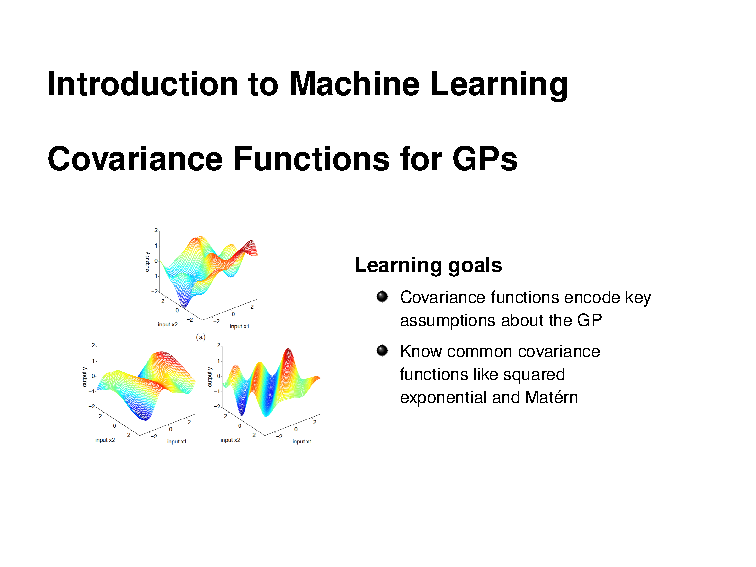
\includepdf[pages=-]{../slides-pdf/slides-gp-covariance.pdf}
\subsection{Gaussian Processes - Prediction}
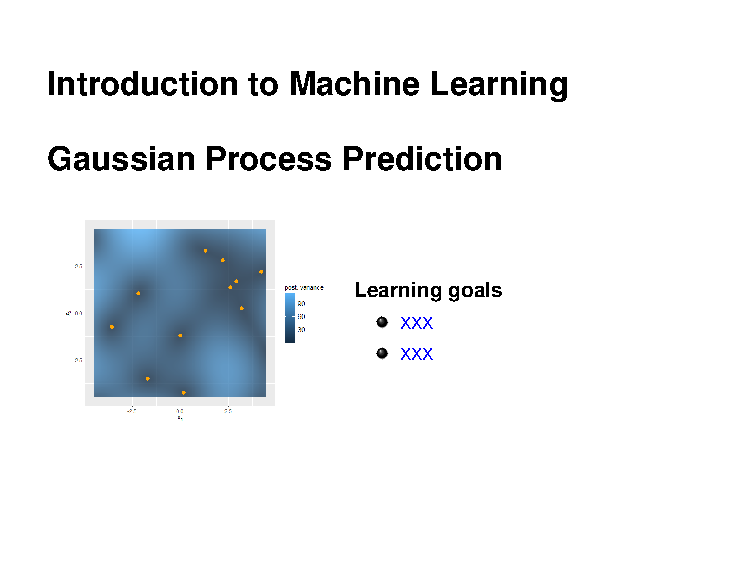
\includepdf[pages=-]{../slides-pdf/slides-gp-prediction.pdf}
\subsection{Gaussian Processes - Training}
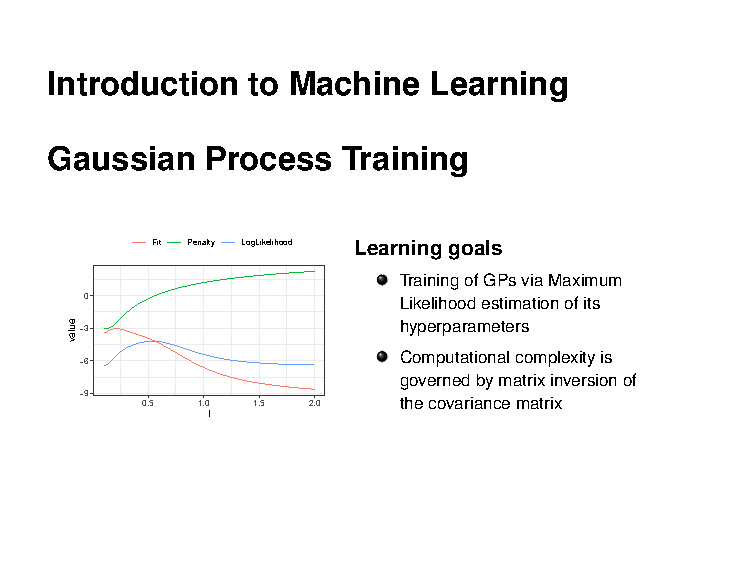
\includepdf[pages=-]{../slides-pdf/slides-gp-training.pdf}
\subsection{Gaussian Processes - Mean}
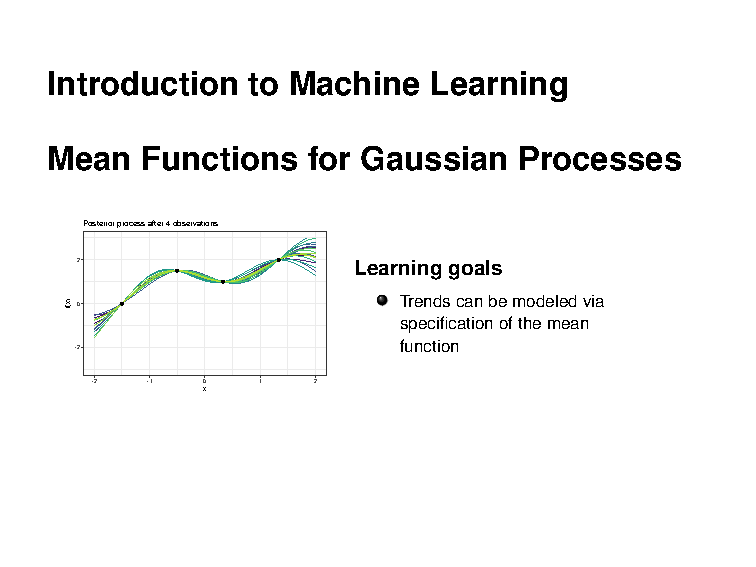
\includepdf[pages=-]{../slides-pdf/slides-gp-mean.pdf}


\section{Supervised Classification}
%Suggested order of slides
% slides-bayes-lm.tex
% slides-gp-basic.tex
% slides-gp-covariance.tex
% slides-gp-prediction.tex
% slides-gp-training.tex
% slides-gp-mean.tex

% not included: 
% slides-x-covariance-adv.tex
% slides-x-gp-additional.tex
% slides-x-gp-classification.tex

\subsection{Bayes LM}
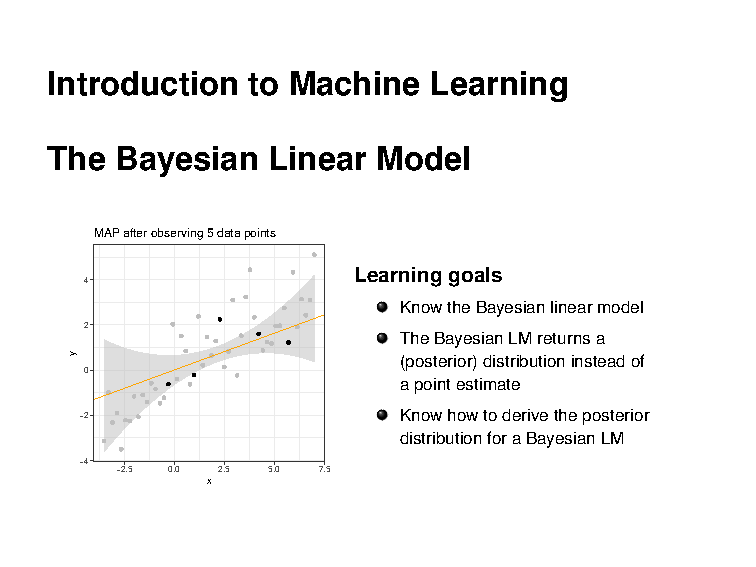
\includepdf[pages=-]{../slides-pdf/slides-gp-bayes-lm.pdf}
\subsection{Gaussian Processes - Basics}
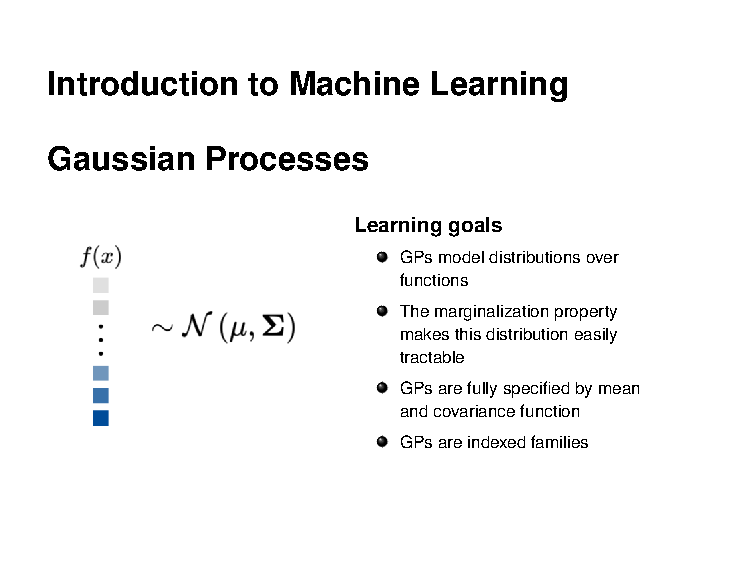
\includepdf[pages=-]{../slides-pdf/slides-gp-basic.pdf}
\subsection{Gaussian Processes - Covariance}
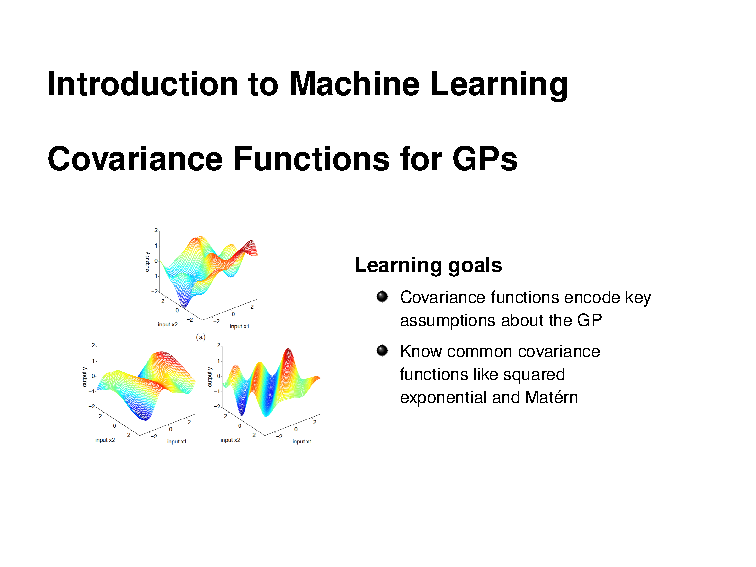
\includepdf[pages=-]{../slides-pdf/slides-gp-covariance.pdf}
\subsection{Gaussian Processes - Prediction}
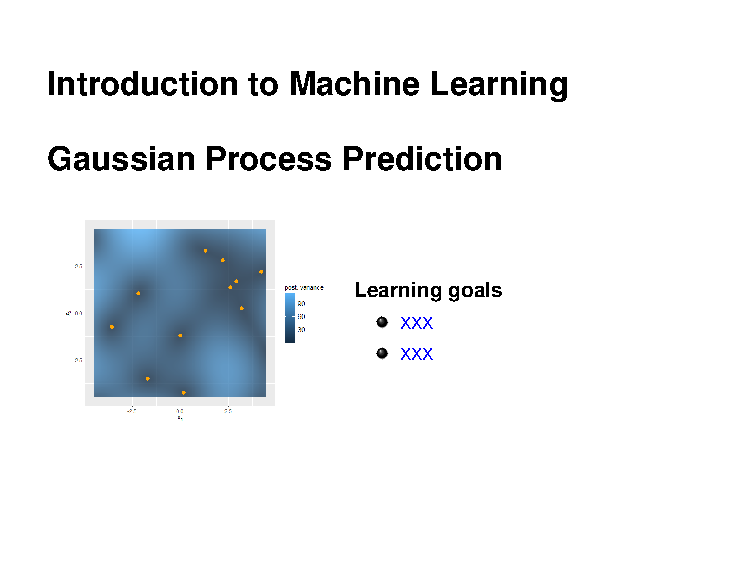
\includepdf[pages=-]{../slides-pdf/slides-gp-prediction.pdf}
\subsection{Gaussian Processes - Training}
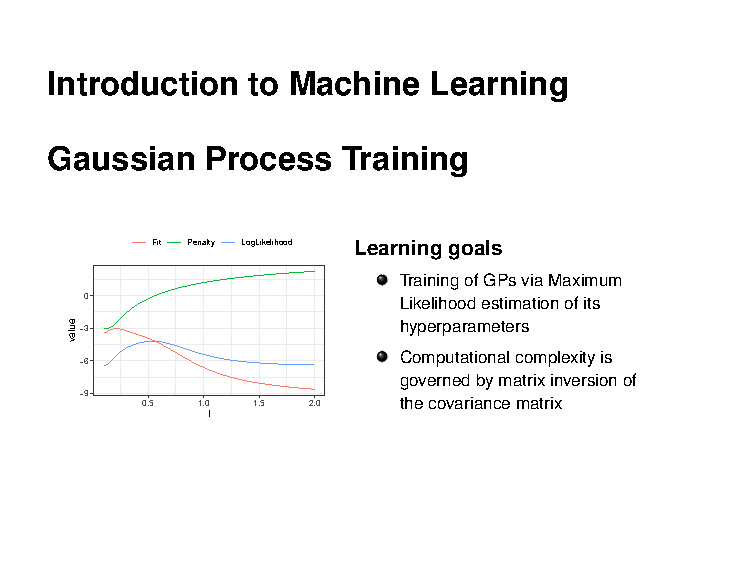
\includepdf[pages=-]{../slides-pdf/slides-gp-training.pdf}
\subsection{Gaussian Processes - Mean}
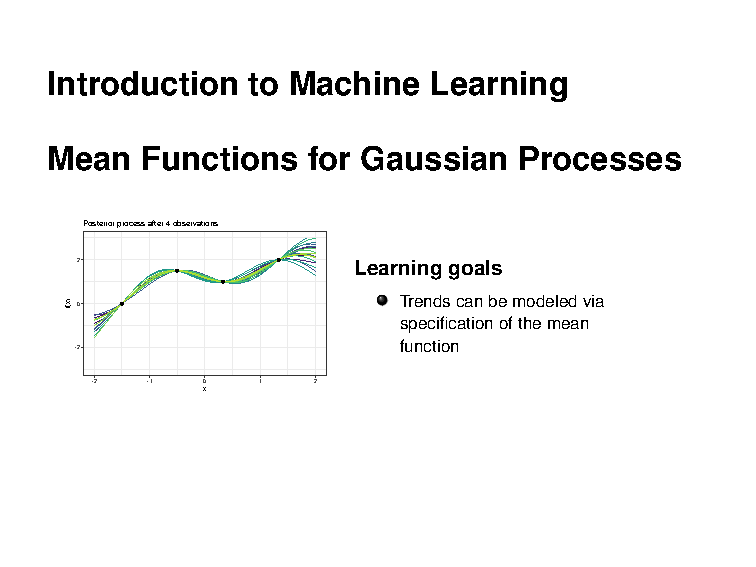
\includepdf[pages=-]{../slides-pdf/slides-gp-mean.pdf}


\section{Performance Evaluation}
%Suggested order of slides
% slides-bayes-lm.tex
% slides-gp-basic.tex
% slides-gp-covariance.tex
% slides-gp-prediction.tex
% slides-gp-training.tex
% slides-gp-mean.tex

% not included: 
% slides-x-covariance-adv.tex
% slides-x-gp-additional.tex
% slides-x-gp-classification.tex

\subsection{Bayes LM}
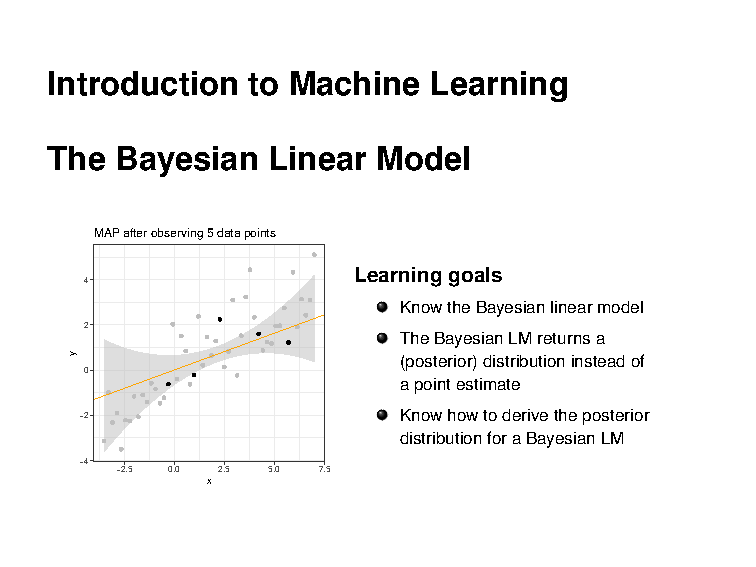
\includepdf[pages=-]{../slides-pdf/slides-gp-bayes-lm.pdf}
\subsection{Gaussian Processes - Basics}
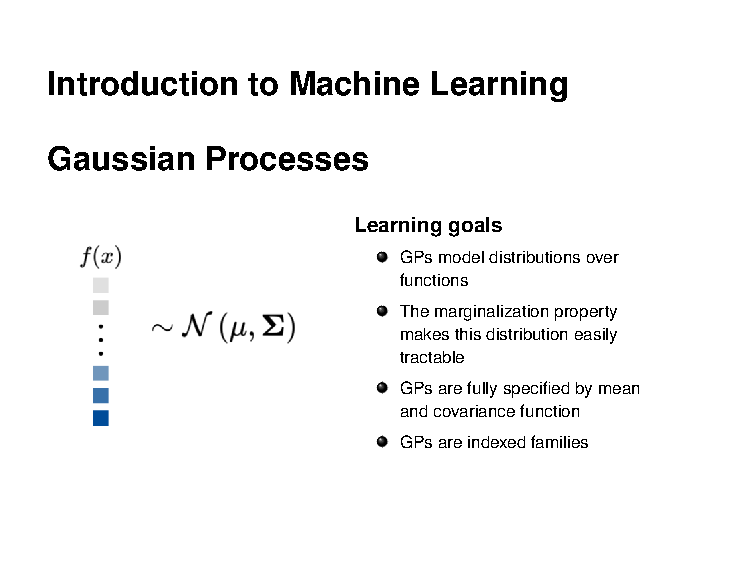
\includepdf[pages=-]{../slides-pdf/slides-gp-basic.pdf}
\subsection{Gaussian Processes - Covariance}
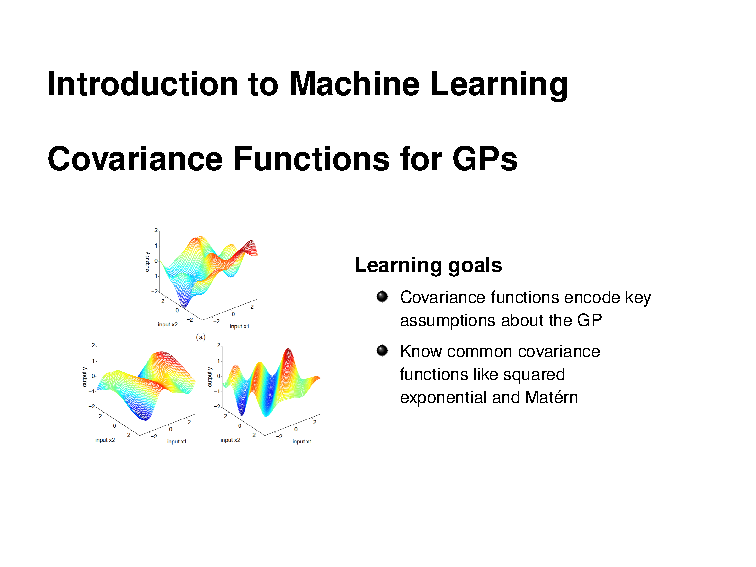
\includepdf[pages=-]{../slides-pdf/slides-gp-covariance.pdf}
\subsection{Gaussian Processes - Prediction}
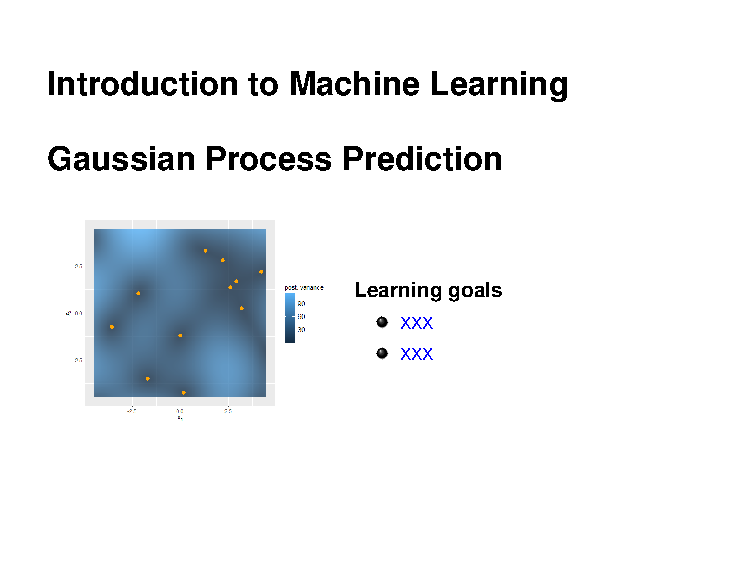
\includepdf[pages=-]{../slides-pdf/slides-gp-prediction.pdf}
\subsection{Gaussian Processes - Training}
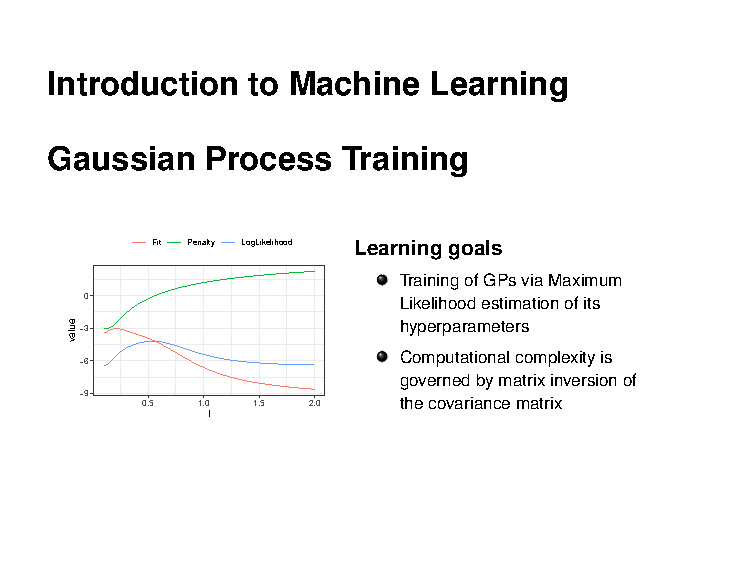
\includepdf[pages=-]{../slides-pdf/slides-gp-training.pdf}
\subsection{Gaussian Processes - Mean}
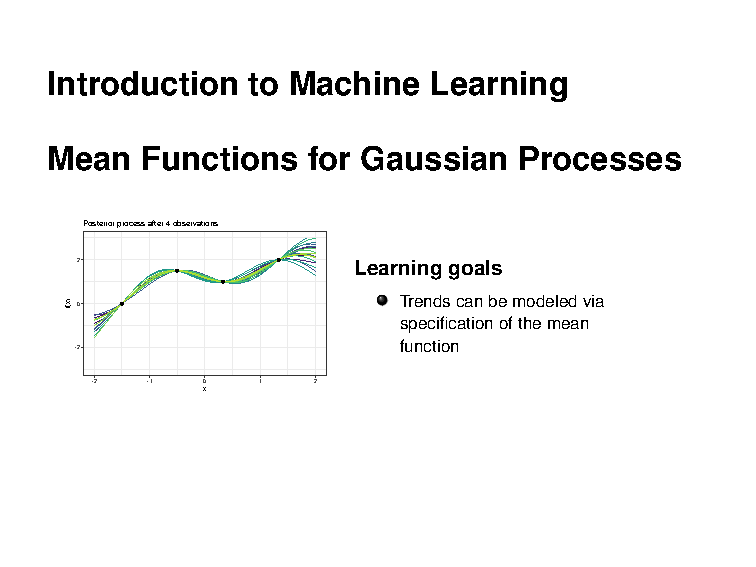
\includepdf[pages=-]{../slides-pdf/slides-gp-mean.pdf}


\section{k-NN}
%Suggested order of slides
% slides-bayes-lm.tex
% slides-gp-basic.tex
% slides-gp-covariance.tex
% slides-gp-prediction.tex
% slides-gp-training.tex
% slides-gp-mean.tex

% not included: 
% slides-x-covariance-adv.tex
% slides-x-gp-additional.tex
% slides-x-gp-classification.tex

\subsection{Bayes LM}
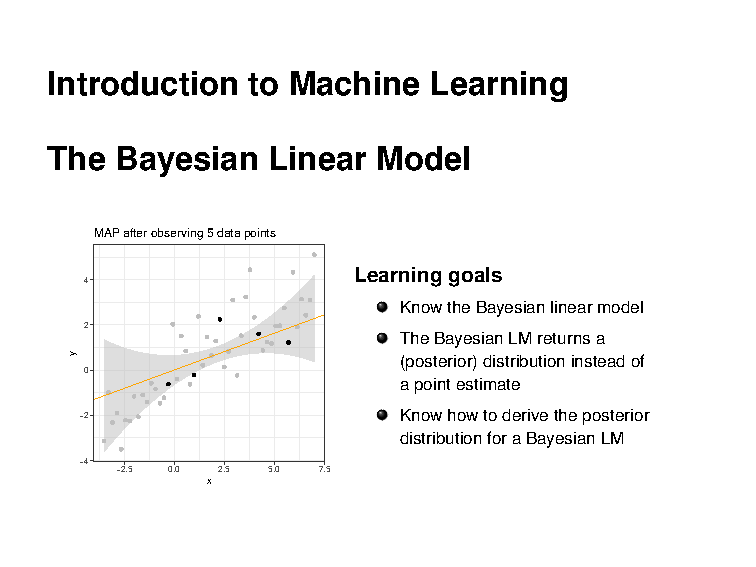
\includepdf[pages=-]{../slides-pdf/slides-gp-bayes-lm.pdf}
\subsection{Gaussian Processes - Basics}
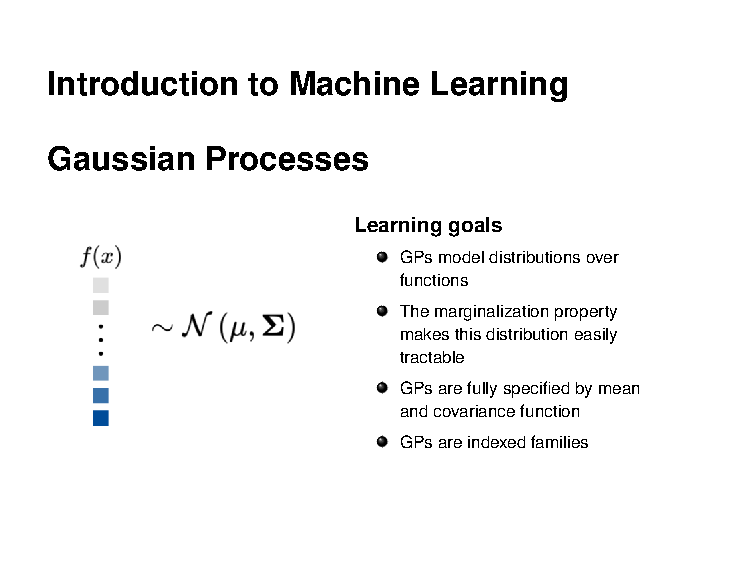
\includepdf[pages=-]{../slides-pdf/slides-gp-basic.pdf}
\subsection{Gaussian Processes - Covariance}
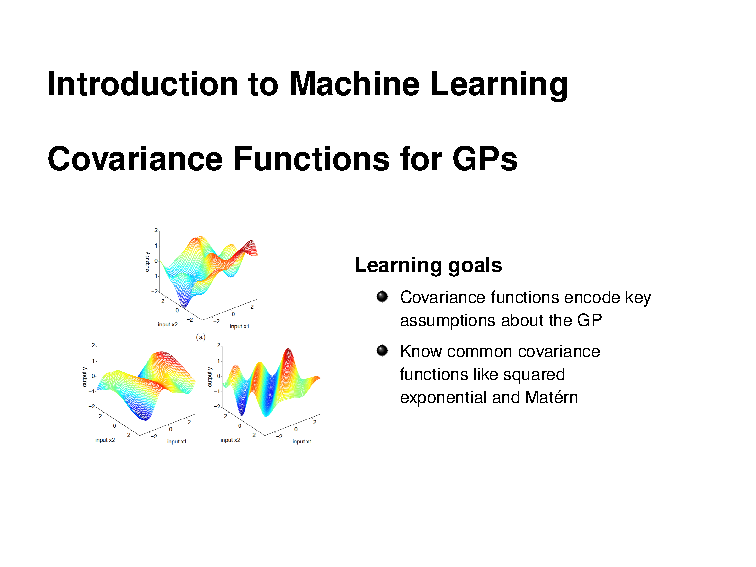
\includepdf[pages=-]{../slides-pdf/slides-gp-covariance.pdf}
\subsection{Gaussian Processes - Prediction}
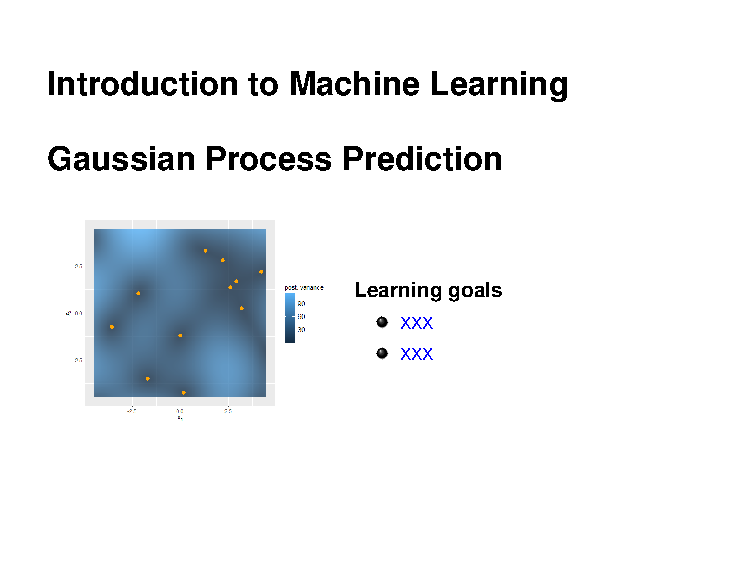
\includepdf[pages=-]{../slides-pdf/slides-gp-prediction.pdf}
\subsection{Gaussian Processes - Training}
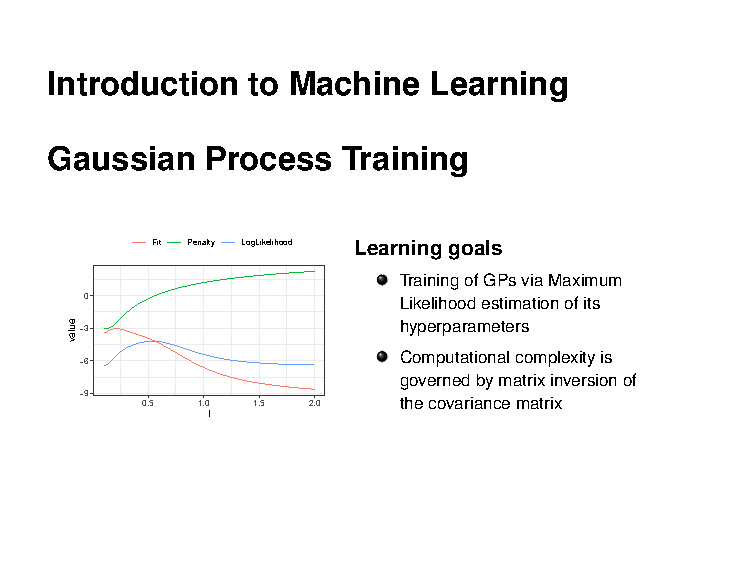
\includepdf[pages=-]{../slides-pdf/slides-gp-training.pdf}
\subsection{Gaussian Processes - Mean}
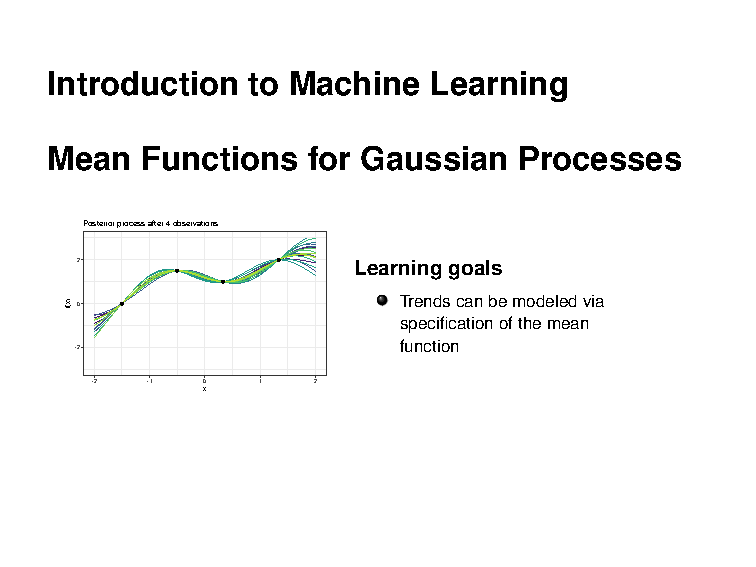
\includepdf[pages=-]{../slides-pdf/slides-gp-mean.pdf}


\section{Classification and Regression Trees (CART)}
%Suggested order of slides
% slides-bayes-lm.tex
% slides-gp-basic.tex
% slides-gp-covariance.tex
% slides-gp-prediction.tex
% slides-gp-training.tex
% slides-gp-mean.tex

% not included: 
% slides-x-covariance-adv.tex
% slides-x-gp-additional.tex
% slides-x-gp-classification.tex

\subsection{Bayes LM}
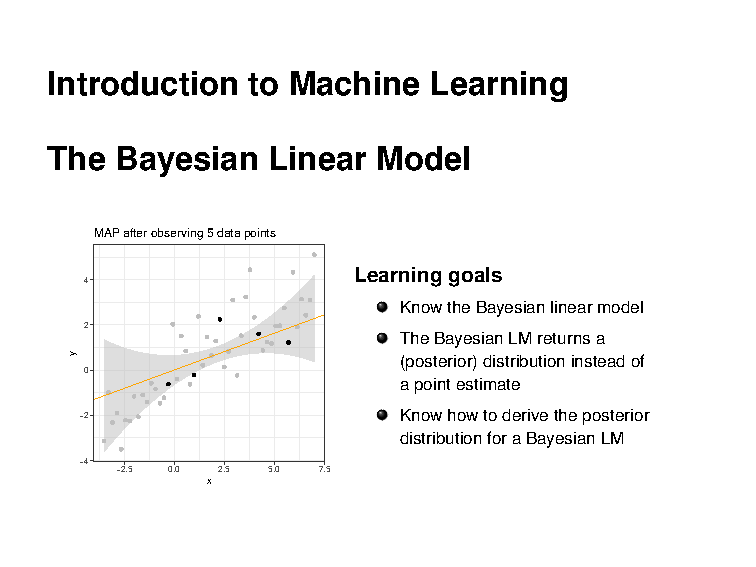
\includepdf[pages=-]{../slides-pdf/slides-gp-bayes-lm.pdf}
\subsection{Gaussian Processes - Basics}
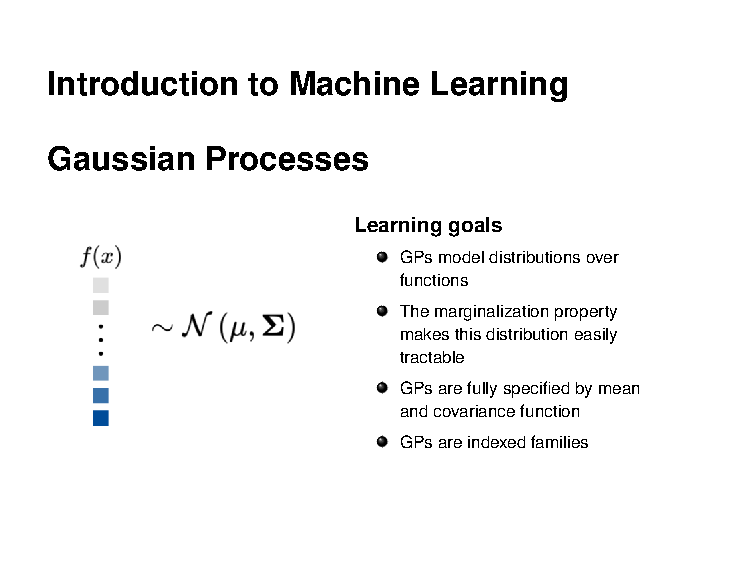
\includepdf[pages=-]{../slides-pdf/slides-gp-basic.pdf}
\subsection{Gaussian Processes - Covariance}
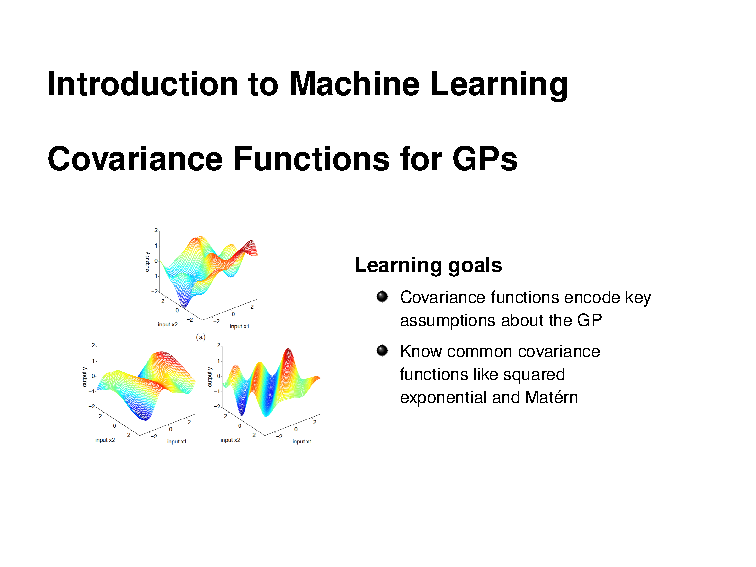
\includepdf[pages=-]{../slides-pdf/slides-gp-covariance.pdf}
\subsection{Gaussian Processes - Prediction}
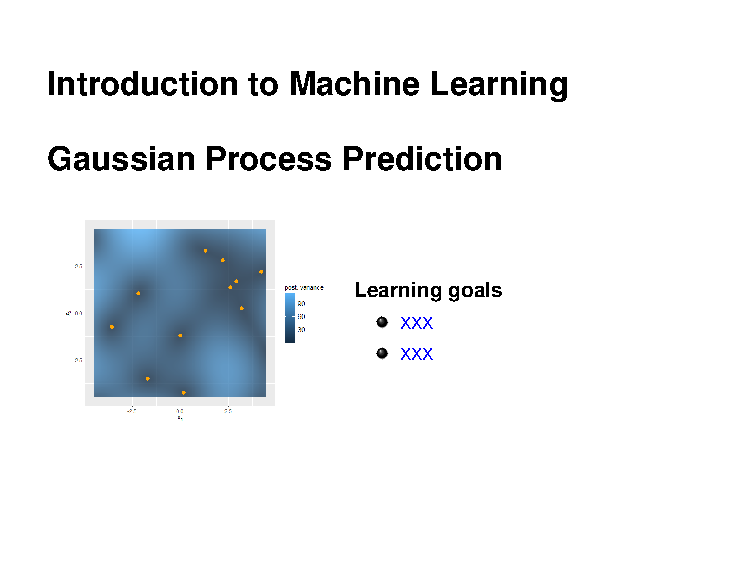
\includepdf[pages=-]{../slides-pdf/slides-gp-prediction.pdf}
\subsection{Gaussian Processes - Training}
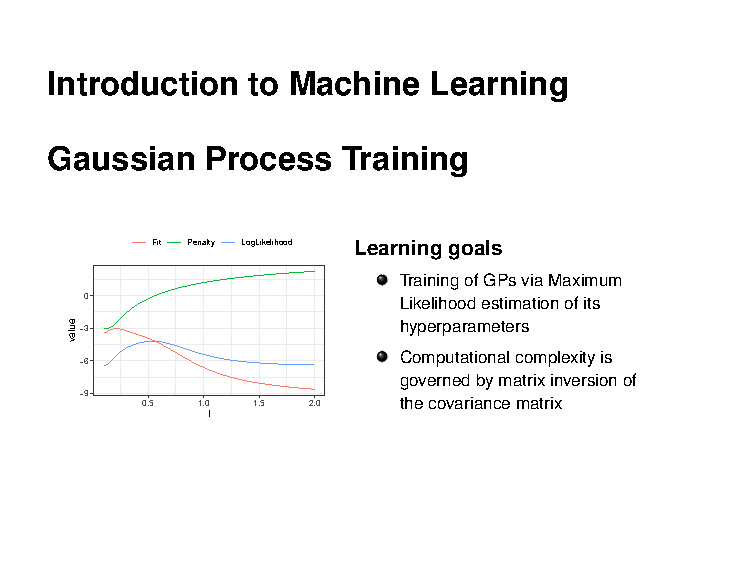
\includepdf[pages=-]{../slides-pdf/slides-gp-training.pdf}
\subsection{Gaussian Processes - Mean}
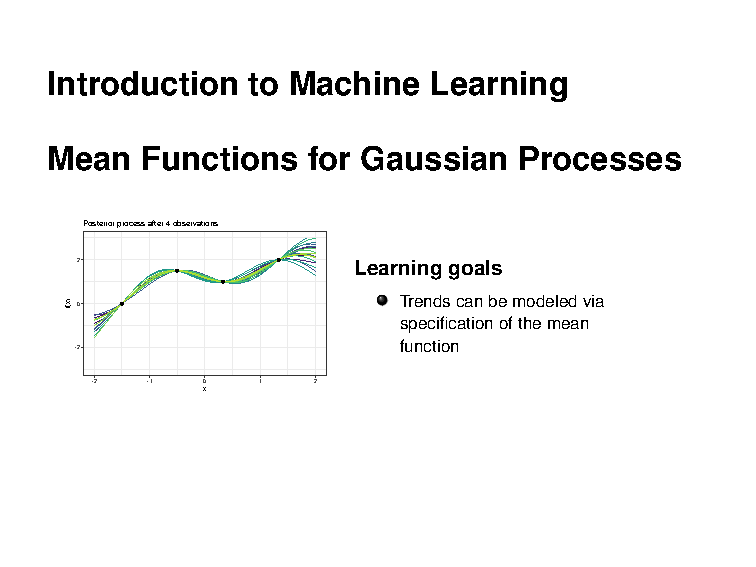
\includepdf[pages=-]{../slides-pdf/slides-gp-mean.pdf}


\section{Random Forests}
%Suggested order of slides
% slides-bayes-lm.tex
% slides-gp-basic.tex
% slides-gp-covariance.tex
% slides-gp-prediction.tex
% slides-gp-training.tex
% slides-gp-mean.tex

% not included: 
% slides-x-covariance-adv.tex
% slides-x-gp-additional.tex
% slides-x-gp-classification.tex

\subsection{Bayes LM}
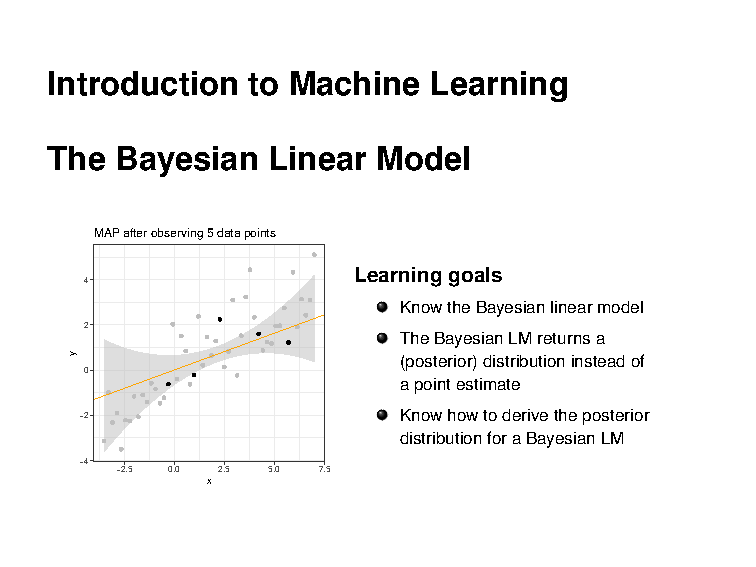
\includepdf[pages=-]{../slides-pdf/slides-gp-bayes-lm.pdf}
\subsection{Gaussian Processes - Basics}
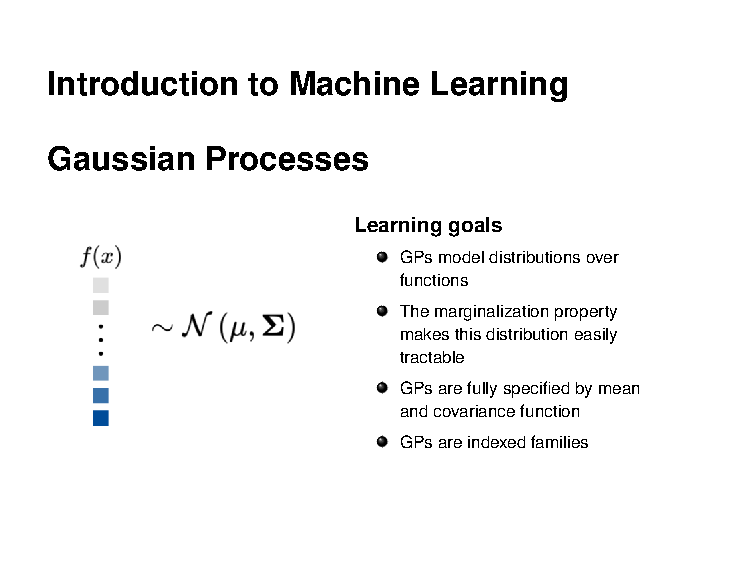
\includepdf[pages=-]{../slides-pdf/slides-gp-basic.pdf}
\subsection{Gaussian Processes - Covariance}
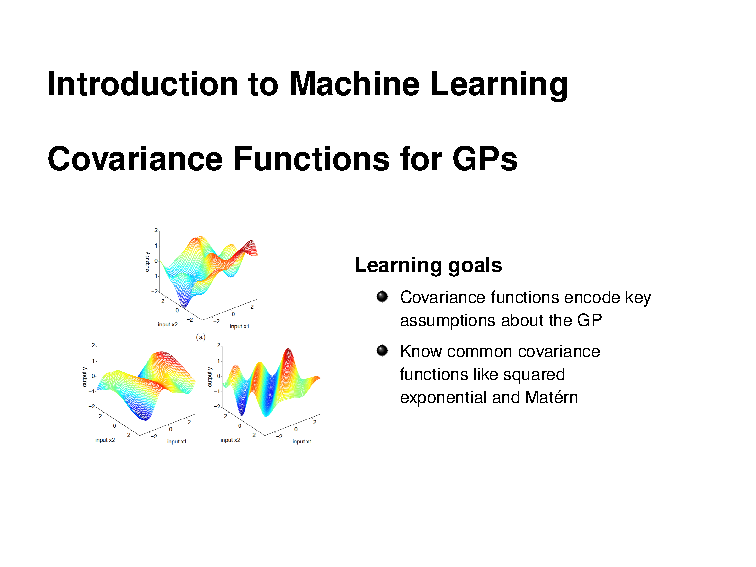
\includepdf[pages=-]{../slides-pdf/slides-gp-covariance.pdf}
\subsection{Gaussian Processes - Prediction}
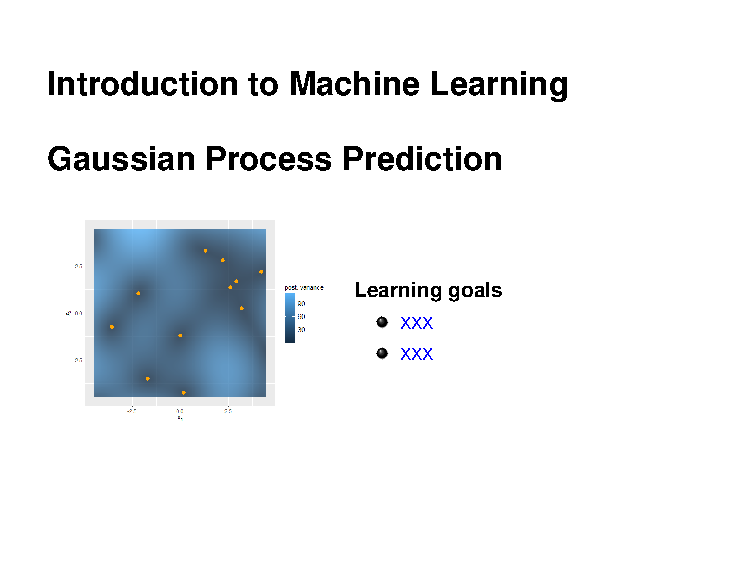
\includepdf[pages=-]{../slides-pdf/slides-gp-prediction.pdf}
\subsection{Gaussian Processes - Training}
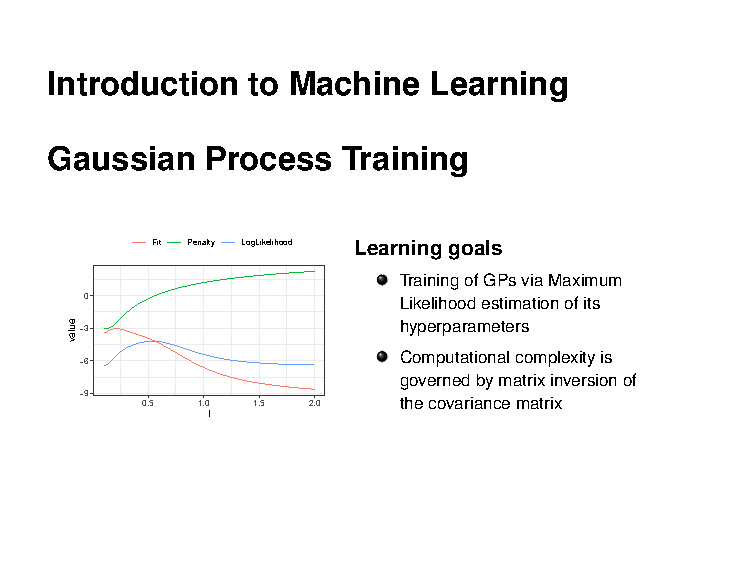
\includepdf[pages=-]{../slides-pdf/slides-gp-training.pdf}
\subsection{Gaussian Processes - Mean}
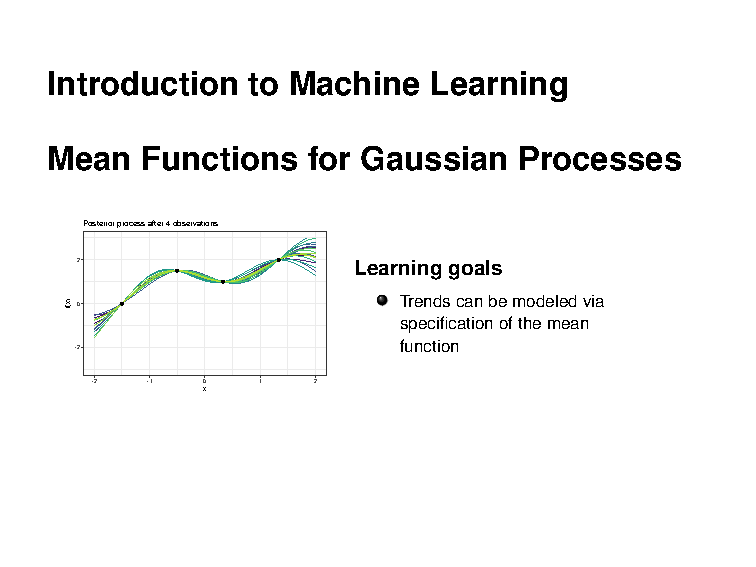
\includepdf[pages=-]{../slides-pdf/slides-gp-mean.pdf}


\section{Neural Networks}
%Suggested order of slides
% slides-bayes-lm.tex
% slides-gp-basic.tex
% slides-gp-covariance.tex
% slides-gp-prediction.tex
% slides-gp-training.tex
% slides-gp-mean.tex

% not included: 
% slides-x-covariance-adv.tex
% slides-x-gp-additional.tex
% slides-x-gp-classification.tex

\subsection{Bayes LM}
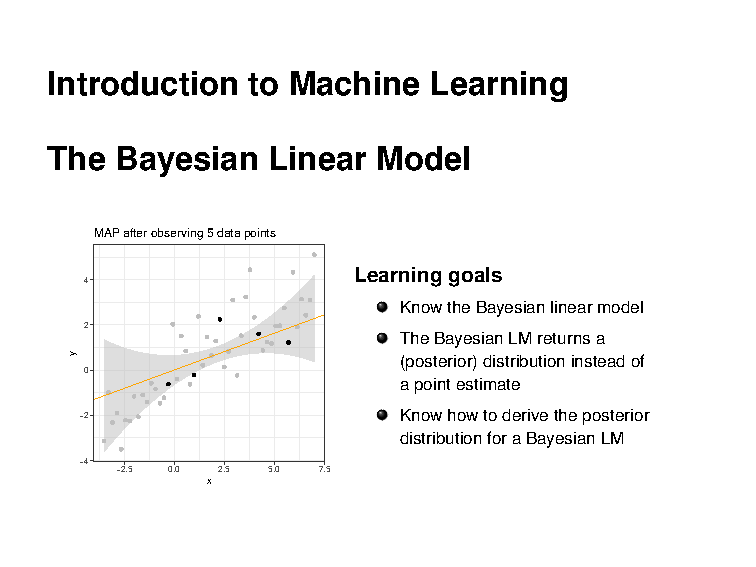
\includepdf[pages=-]{../slides-pdf/slides-gp-bayes-lm.pdf}
\subsection{Gaussian Processes - Basics}
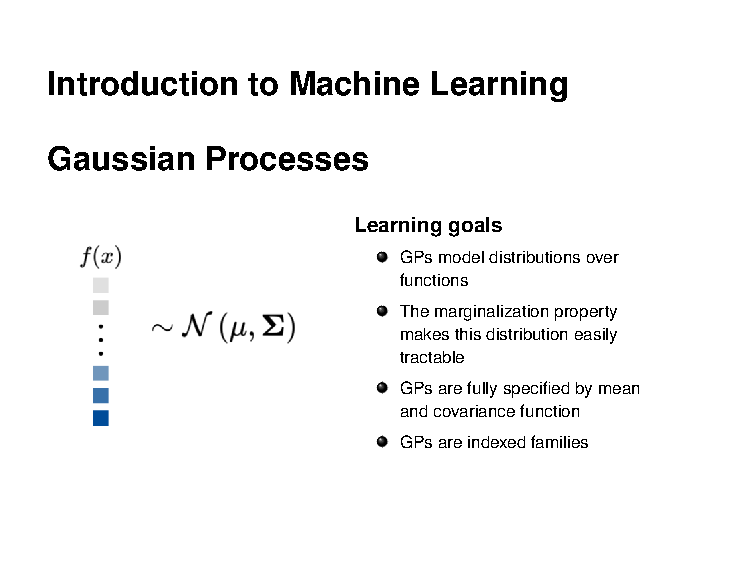
\includepdf[pages=-]{../slides-pdf/slides-gp-basic.pdf}
\subsection{Gaussian Processes - Covariance}
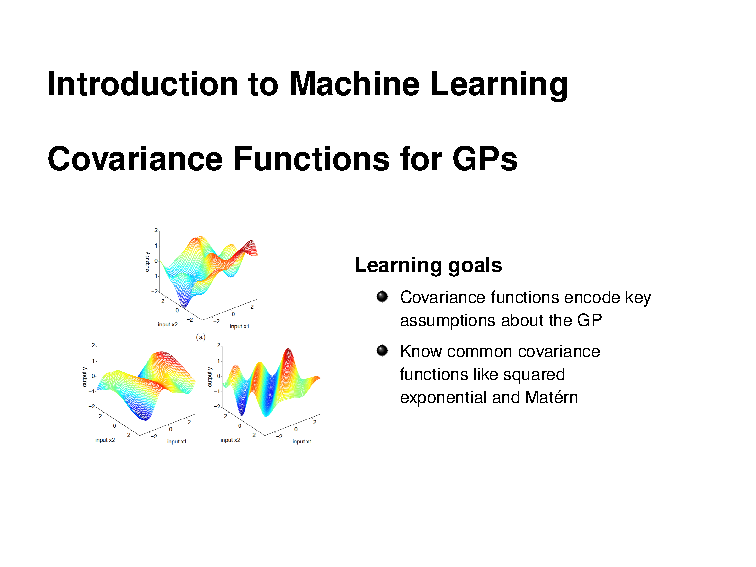
\includepdf[pages=-]{../slides-pdf/slides-gp-covariance.pdf}
\subsection{Gaussian Processes - Prediction}
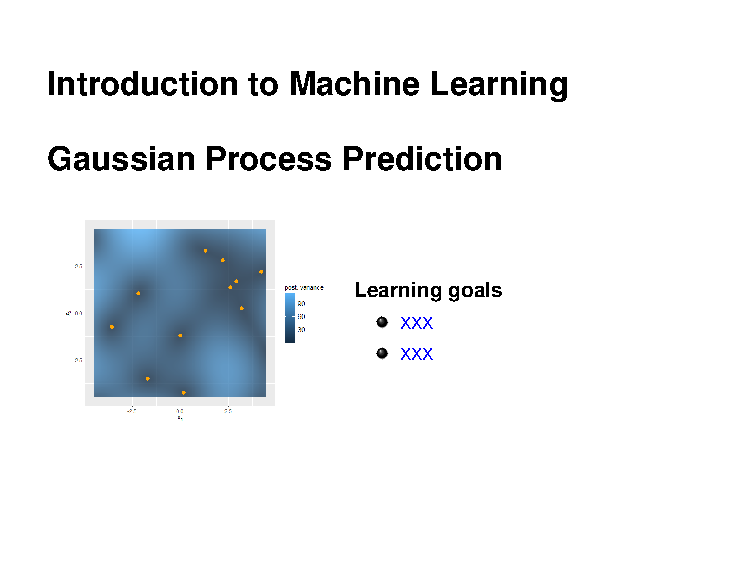
\includepdf[pages=-]{../slides-pdf/slides-gp-prediction.pdf}
\subsection{Gaussian Processes - Training}
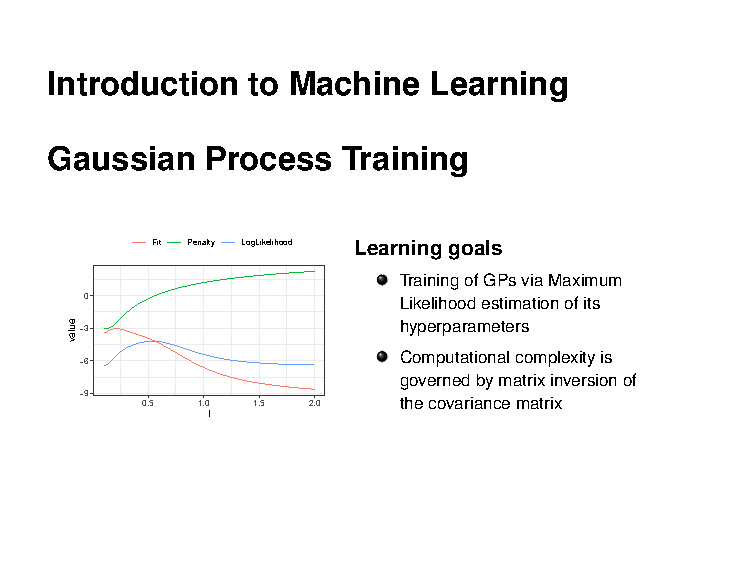
\includepdf[pages=-]{../slides-pdf/slides-gp-training.pdf}
\subsection{Gaussian Processes - Mean}
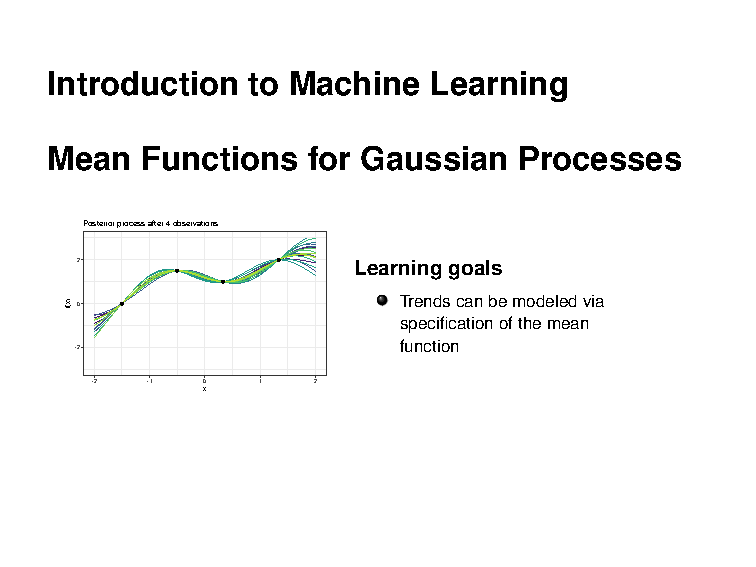
\includepdf[pages=-]{../slides-pdf/slides-gp-mean.pdf}


\section{Tuning}
%Suggested order of slides
% slides-bayes-lm.tex
% slides-gp-basic.tex
% slides-gp-covariance.tex
% slides-gp-prediction.tex
% slides-gp-training.tex
% slides-gp-mean.tex

% not included: 
% slides-x-covariance-adv.tex
% slides-x-gp-additional.tex
% slides-x-gp-classification.tex

\subsection{Bayes LM}
\includepdf[pages=-]{../slides-pdf/slides-gp-bayes-lm.pdf}
\subsection{Gaussian Processes - Basics}
\includepdf[pages=-]{../slides-pdf/slides-gp-basic.pdf}
\subsection{Gaussian Processes - Covariance}
\includepdf[pages=-]{../slides-pdf/slides-gp-covariance.pdf}
\subsection{Gaussian Processes - Prediction}
\includepdf[pages=-]{../slides-pdf/slides-gp-prediction.pdf}
\subsection{Gaussian Processes - Training}
\includepdf[pages=-]{../slides-pdf/slides-gp-training.pdf}
\subsection{Gaussian Processes - Mean}
\includepdf[pages=-]{../slides-pdf/slides-gp-mean.pdf}


\section{Nested Resampling}
%Suggested order of slides
% slides-bayes-lm.tex
% slides-gp-basic.tex
% slides-gp-covariance.tex
% slides-gp-prediction.tex
% slides-gp-training.tex
% slides-gp-mean.tex

% not included: 
% slides-x-covariance-adv.tex
% slides-x-gp-additional.tex
% slides-x-gp-classification.tex

\subsection{Bayes LM}
\includepdf[pages=-]{../slides-pdf/slides-gp-bayes-lm.pdf}
\subsection{Gaussian Processes - Basics}
\includepdf[pages=-]{../slides-pdf/slides-gp-basic.pdf}
\subsection{Gaussian Processes - Covariance}
\includepdf[pages=-]{../slides-pdf/slides-gp-covariance.pdf}
\subsection{Gaussian Processes - Prediction}
\includepdf[pages=-]{../slides-pdf/slides-gp-prediction.pdf}
\subsection{Gaussian Processes - Training}
\includepdf[pages=-]{../slides-pdf/slides-gp-training.pdf}
\subsection{Gaussian Processes - Mean}
\includepdf[pages=-]{../slides-pdf/slides-gp-mean.pdf}


%\section{mlr3}
%%Suggested order of slides
% slides-bayes-lm.tex
% slides-gp-basic.tex
% slides-gp-covariance.tex
% slides-gp-prediction.tex
% slides-gp-training.tex
% slides-gp-mean.tex

% not included: 
% slides-x-covariance-adv.tex
% slides-x-gp-additional.tex
% slides-x-gp-classification.tex

\subsection{Bayes LM}
\includepdf[pages=-]{../slides-pdf/slides-gp-bayes-lm.pdf}
\subsection{Gaussian Processes - Basics}
\includepdf[pages=-]{../slides-pdf/slides-gp-basic.pdf}
\subsection{Gaussian Processes - Covariance}
\includepdf[pages=-]{../slides-pdf/slides-gp-covariance.pdf}
\subsection{Gaussian Processes - Prediction}
\includepdf[pages=-]{../slides-pdf/slides-gp-prediction.pdf}
\subsection{Gaussian Processes - Training}
\includepdf[pages=-]{../slides-pdf/slides-gp-training.pdf}
\subsection{Gaussian Processes - Mean}
\includepdf[pages=-]{../slides-pdf/slides-gp-mean.pdf}


\end{document}
  
